\documentclass[svgnames]{uvamscse} %Add xcolor parameter here to prevent conflict.

\usepackage[utf8]{inputenc}
\usepackage[english]{babel}
\usepackage{booktabs}
\usepackage{array}
\usepackage{paralist}
\usepackage{longtable}
\usepackage{amsmath,amssymb,amsthm}
\usepackage{csquotes}
\usepackage{xcolor}
\usepackage{framed}
\usepackage{listings}
\usepackage[backend=biber,style=numeric]{biblatex}
\usepackage[colorinlistoftodos]{todonotes}
\usepackage{pgfgantt}
\usepackage{hyperref}
\usepackage[toc,acronym,nogroupskip,nohypertypes={acronym}]{glossaries}

\colorlet{shadecolor}{yellow}

%Title page
\title{Improving management and maintainability of virtual container networks through CNI}
\author{Willem Jan Glerum - 11317493}
\authemail{wjglerum@gmail.com}
\host{Lunatech Labs B.V. \url{https://lunatech.com} }
\supervisor{Dr. Paola Grosso\ --\ UvA}
\date{\today}
%Random virtual network image
\coverpic[200pt]{images/virtual.png}

\abstract{
  This section summarises the content of the thesis for potential readers who do not have time to read it whole,
  or for those undecided whether to read it at all. Sum up the following aspects:

  \begin{itemize}
    \item relevance and motivation for the research
    \item research questions and a brief description of the research method
    \item results, contributions and conclusions
  \end{itemize}
}

%Styles for the lstlisting blocks.
%\input{lststyles}

%Glossary register:
\newacronym{cni}{CNI}{Container Network Interface}
\newacronym{sdn}{SDN}{Software Defined Networking}
\newacronym{poc}{PoC}{Proof of Concept}
\newacronym{ucr}{UCR}{Universal Container Runtime}
\newacronym{iot}{IoT}{Internet of Things}
\newacronym{dcos}{DC/OS}{The Datacenter Operating System}
\newacronym{vm}{VM}{Virtual Machine}
\newacronym{os}{OS}{Operating System}
\newacronym{aws}{AWS}{Amazon Web Services}
\newacronym{gcp}{GCP}{Google Cloud Platform}
\newacronym{ipam}{IPAM}{IP Address Management}
\newacronym{api}{API}{Application Programming Interface}
\newacronym{http}{HTTP}{Hypertext Transfer Protocol}
\newacronym{grpc}{gRPC}{gRPC Remote Procedure Calls}
\newacronym{bpf}{BPF}{Berkeley Packet Filter}
\newacronym{jit}{JIT}{Just In Time}
\newacronym{bgp}{BGP}{Border Gateway Protocol}
\newacronym{bird}{BIRD}{BIRD Internet Routing Daemon}
\newacronym{nat}{NAT}{Network Address Translation}
\newacronym{ip}{IP address}{Internet Protocol address}
\newacronym{dhcp}{DHCP}{Dynamic Host Configuration Protocol}
\newacronym{vlan}{VLAN}{Virtual LAN}
\newacronym{cgroup}{cgroup}{Control Group}
\newacronym{vxlan}{VXLAN}{Virtual Extensible LAN}


%Bibliography DB
\addbibresource{refs.bib}

%Useful definitions for (long)tables:
\newcolumntype{L}[1]{>{\raggedright\let\newline\\\arraybackslash\hspace{0pt}}p{#1}}
\newcolumntype{C}[1]{>{\centering\let\newline\\\arraybackslash\hspace{0pt}}p{#1}}
\newcolumntype{R}[1]{>{\raggedleft\let\newline\\\arraybackslash\hspace{0pt}}p{#1}}

\begin{document}

\maketitle
\chapter{Introduction}
\label{chap:introduction}

\chapter{Problem statement and motivation}
\emph{You describe in detail what problem the research is addressing,
and what is the motivation to address this problem. There is a concise and objective
statement of the research questions, hypotheses and goals. It is made clear why these questions
and goals are important and relevant to the world outside the university (assuming it exists).
You can already split the main research question into subquestions in this chapter. This section
also describes an analysis of the problem: where does it occur and how, how often, and what are
the consequences? An important part is also to scope the research: what aspects are included
and what aspects are deliberately left out, and why?}

This chapter aims to explain the why of this thesis. First we explore and explain the problems with managing virtual container networks, next we elaborate on the motivation for this thesis. Last we introduce the research questions and explain why these are relevant.

\section{Problem statement}
At the moment applications are moved from legacy deployments to container deployments. A container is a set of isolated processes and application dependencies that are packaged together in an image. This image can run locally on a developers machine or on a container orchestration platform in production. Containers are more flexible opposed to \glspl{vm} as you do not need to run and boot an entire \gls{os}. The most well known system for running containers locally is Docker\footnote{\url{https://www.docker.com/}}. To make applications highly available people make use of a container orchestration platform like Kubernetes\footnote{\url{https://kubernetes.io/}} or \gls{dcos}\footnote{\url{https://dcos.io/}} to allow scaling of those containers. Cloud providers such as \gls{aws}\footnote{\url{https://aws.amazon.com//}} and \gls{gcp}\footnote{\url{https://cloud.google.com/}} even enable you to run containers without worrying about the underlying infrastructure. \todo[inline]{Do I cite or use a footnote for referencing to all those technologies??? Having all the footnotes seems messy, but a citation might be too much??}

In production workloads operators want to isolate applications, the traditional way is to use firewall policies and different physical networks between applications in a datacenter. For containers operators need to be more flexible as workloads change all the time. Therefore they introduced a form of \gls{sdn} to create virtual networks within a container orchestration platform.  There are different implementations and vendors providing virtual networks and policies, such as Project Calico\footnote{\url{https://projectcalico.org/}}\cite{calico} and Cilium\footnote{\url{https://cilium.io/}}. These plugins are standardised with the \gls{cni}\footnote{\url{https://github.com/containernetworking/cni}} standard, a set of specifications and plugins for configuring networks. \Gls{cni} allows you to chain different plugins together, for example for \gls{ipam}, overlay networks and network policies.

The focus will be on \gls{dcos} and Calico as one of Lunatech's clients uses those technologies for their container orchestration. The client wants to isolate workloads from different tenants within their organisation and logically split workloads in the data processing pipeline. Currently there is no way for an operator of a cluster to see and manage the virtual networks and policies in \gls{dcos} as each \gls{cni} plugin uses its own control plane. An operator must reach down the host machine to inspect the network configuration. To allow easy administration and maintainability we need a solution to at least get an overview of the network and be able to inspect those. Thus there is no easy way for the client to check if workloads are really isolated. 
\section{Motivation}
When there is visibility of the implemented networks and policies we can empower administrators with better means to manage and maintain the virtual networks on a container orchestration platform. Allowing a developer to simply allow or deny traffic between different applications are namespaces. This can be achieved by erasing the differences between the \gls{cni} plugins and hiding their complexity from them. As an extensions we could also automatically provision new \gls{cni} plugins to help operators create new network services in a flexible manner, without worrying about the concrete implementation details.

On a container orchestration platform we also need an ingress point to allow traffic to the container workloads. This involves for example configuring loadbalancers on your cloud platform. However when something changes on the container orchestration level, an operator must also update the relevant loadbalancers to redirect the traffic to the correct container. This is also called North-South traffic, East-West traffic is within the cluster when for example a pool of webservers talk to a pool of applications servers. The applications servers could be on a different virtual network, protected by network policies and need to be load-balanced.

Furthermore when this is in place we can also look at automating the tasks of administrator as much as possible. Here we could think of self-adapting networks, where the system detects a sub-optimal solution and applies the new configuration in place, with or without the confirmation of the operator. Often it is the case that a firewall rule is blocking traffic, it can be very hard for an application developer who wants to deploy his application to find the exact problem, as his application works fine on his local machine. A visualisation can be created to help an operator to gain insight of the applied network policies, allowing to find the problematic policy faster in an interactive process. Self adapting networks and visualisations are outside the scope of this thesis, as we first need a way of exposing the current network infrastructure. When everything is in place it becomes easier to think of new use cases and ways to help operators and developers to debug the cluster and the applied policies.


\section{Research questions}
The following research questions were raised during the formulation of this assignment:
\begin{itemize}
    \item \textbf{Q1} What are the current problems in maintaining virtual container networks and how do different vendors address this issue?
    \item \textbf{Q2} How can the maintainability of virtual container networks be improved through \gls{cni}?   
\end{itemize}

\subsection{Research question 1}
First we need to know what the problems are in in the current solutions with managing and maintaining virtual networks, before we propose a solution. This can be based on the direct experience of people within the client's project and/or information found online or in previous research. Furthmore we could look what other providers are doing to address this issue. At the moment Kubernetes is very popular and adapted by a lot of companies and developers. We could learn from their experience and mistakes.

\subsection{Research question 2}
This questions aims to find a solution for the concrete problems found with the first question. To prevent reinventing the wheel we should critically asses if we can reuse some of the solutions from other providers or standards. And of course see if we can improve the current situation by suggesting a new solution.

%\chapter{Research method}

\chapter{Background and context}
\emph{This chapter contains all the information needed to put the thesis into
context. It is common to use a revised version of your literature survey for this purpose. It
is important to explicitly refer from your text to sources you have used, they will be listed in
your bibliography.}
\chapter{Research}
%\emph{This chapter reports on the execution of the research method as described in an earlier chapter. If the research has been divided into phases, they are introduced, reported on and concluded individually. If needed, this chapter could be split up to balance out the sizes of all chapters.}
This chapter reports on the execution of the research to demonstrate what has been done. First we explain the current difficulties with managing virtual networks on \gls{dcos}. Next we explore the approach how another popular container orchestration platform, Kubernetes, handles virtual networks. Last we explain the approach we took to build the \gls{poc}.

\section{Current state of virtual networks in DC/OS}
\Gls{dcos} provides virtual networks by itself as overlay networks which can be used by the Docker and Mesos containerizer. This overlay is prepacked and enabled by default on the cluster. \Gls{cni} plugins are also supported on \gls{dcos} and can be used by both containerizers.

\subsection{DC/OS virutal networks}
The overlay network was introduced to enable an IP-per-container model in \gls{dcos}. This allows operators to run applications on the default ports without worrying about port conflicts. This is done by creating an overlay network using \gls{vxlan}\cite{mahalingam2014virtual} which is supported by the Linux kernel. It works by creating two network bridges on each host, one for each containerizer. Containers on the same host and bridge can communicate directly with each other over the network bridge. And a packet from a Mesos container to a Docker container will be routed through both bridges. A packet from a Mesos container on Agent~1 to a Docker container on Agent~2 follows a different path. First the packet will be routed to the Mesos bridge, the host's network stack consumes the package and encapsulates using \gls{vxlan} on Agent~1. Next Agent~2 decapsulates this packet and sends it up to the Docker bridge to be sent to the Docker container as can be seen in Figure~\ref{fig:dcos-overlay-arch}.

IP address are managed by the agent itself instead of a central location. A central location requires a reliably and consistent way of handing IP addresses in the cluster. The default configuration uses a \texttt{9.0.0.0/8} subnet, this will devided in smaller chunks, a \texttt{/24} to be managed by every agent itself. On the agent this subnet is divided into two equal subnets for each containerizer, resulting in 32 usable IP addresses for each container type on every agent.
\begin{figure}
    \centering
    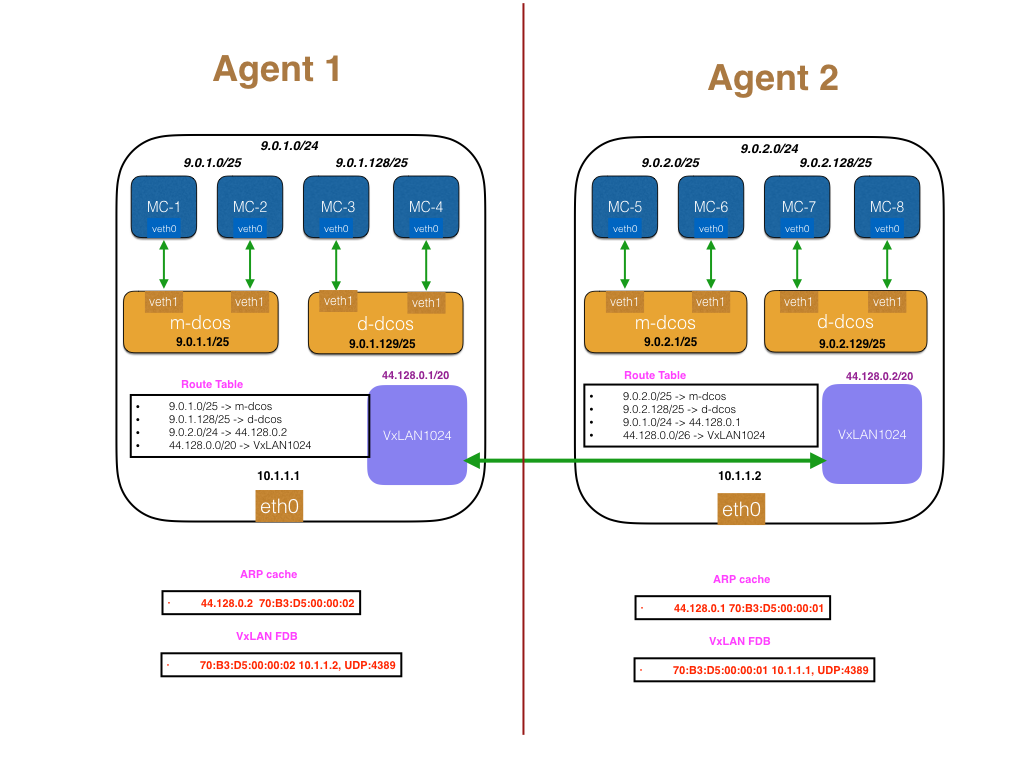
\includegraphics[width=1\columnwidth]{images/dcos-overlay-arch}
    \caption{DC/OS overlay in action\cite{dcos_overlay_arch}}
    \label{fig:dcos-overlay-arch}
\end{figure}

The default overlay network has the following limitations:
\begin{itemize}
    \item A limit on the number of usable IP addresses on each host, determined by the network prefix size. The default maximum is 32 Mesos and 32 Docker containers.
    \item Only IPv6 support for Docker containers, Mesos containers will fail to start.
    \item Operators are only able to create virtual networks during installation, this requires planning on before hand.
    \item The length of network names is limited as the Linux kernel only allows 15 characters for a network interface name.
    \item Marathon cannot execute healhtchecks in the default configurations as Marathon itself is not running on the virtual network.
\end{itemize}

\subsection{CNI plugins on DC/OS}
Too allow for more flexibility with virtual networks operators can also chose to create network with other providers.
\begin{displayquote}
    ``NOTE: The network tab currently displays information about containers that are associated with virtual networks managed by DC/OS overlay. It does not have information about containers running on virtual networks managed by any other CNI/CNM provider.'' %https://docs.mesosphere.com/1.11/networking/SDN/dcos-overlay/#limitations
\end{displayquote}



\subsection{Problems}

\section{Virtual networks in Kubernetes}

\section{Proof of concept}

\chapter{Results}
\emph{This chapter presents and clarifies the results obtained during the research. The focus
should be on the factual results, not the interpretation or discussion. Tables and graphics
should be used to increase the clarity of the results where applicable.}

\chapter{Conclusions}
\label{chap:conclusions}
%\emph{This chapter contains the analysis and interpretation of the results. The research questions are answered as best as possible with the results that were obtained. The analysis also discussed parts of the questions that were left unanswered. An important topic is the validity of the results. What methods of validation were used? Could the results be generalised to other cases? What threats to validity can be identified? There is room here to discuss the results of related scientific literature here as well. How do the results obtained here relate to other work, and what consequences are there? Did your approach work better or worse? Did you learn anything new compared to the already existing body of knowledge? Finally, what could you say in hindsight on the research approach by followed? What could have done better? What lessons have been learned? What could other researchers use from your experience? A separate section should be devoted to future work", i.e., possible extension points of your work that you have identified. Even other researchers should be able to use those as a starting point.}
This thesis describes the difficulties in managing virtual networks on \gls{dcos}. For operators it is possible to create virtual networks using \gls{cni} plugins and some have support for network policies. However there is no central place in \gls{dcos} to see and configure those networks and policies. Unlike in Kubernetes where operators can manage the virtual networks by providing a desired state, the cluster then takes care of configuring the virtual networks and network policies. We first explored the different technologies in use and explained how they all work. This gives us a good foundation to be able to understand the difficulties in managing virtual container networks. Next we conducted a research on the features that are missing to manage those networks and how other vendors such as Kubernetes handle this.

Next a \gls{poc} was built to improve the management of virtual networks on \gls{dcos}. This \gls{poc} demonstrates that it is possible to abstract different \gls{sdn} solutions into one central \gls{api}. This \gls{api} can be used by operators to create new policies regardless of the plugins implemented within the cluster. Furthermore it enables developers to debug and see which policies are blocking traffic to their applications. Giving insight to developers deemed crucial as developers would end up removing their applications from the virtual network to make them work. This is an unwanted situation at Lunatech's automotive client because they need to isolate different parts of their data processing pipeline for privacy and security concerns. The newly built api-server is able to provide useful insights into the state of the network.

To conclude we can say that the new solution improves the management of virtual networks on \gls{dcos}. As operators and developers are able to retrieve and configure the virtual network state from a central place instead of having to dig into the concrete implementations of each \gls{sdn} provider.

\chapter{Discussion}
\label{chap:discussion}

\clearpage
\printbibliography{}

\appendix%
\glsresetall%  Reset acronym tracking. (so reintroduce as "Full (ACR)" in appendices).

%\chapter{Literature}


\end{document}
